\section{Dataset creation}
\label{sec:dataset_creation}
In order to carry out further computational analysis of the topic it is helpful to have an annotated dataset. Since no extensive datasets exist for UMR, I had to create my own. The traditional route of hand-annotating including has been a standard paradigm for many years however is highly time-intensive. Crowdsourcing is a more time- and cost-effective way of creating data, however has been shown to be of variable quality \citep{li2024comparative}, especially when the task requires more expert knowledge. Furthermore, there are a range of biases which can affect data quality \citep{Beck2023}. The huge success of LLMs in recent years has prompted some to look at utilising them for dataset annotation, either combined with human annotators \citep{goel2023llms} or on their own \citep{he2023annollm, llmsForPragAndDiscAnalysis, Gilardi_2023}.

\subsection{Dataset annotation with LLMs}
\citet{törnberg2024best} formulated a set of best practices when using LLMs as text annotators, which I aim to be guided by. The paper provides guidelines for those wishing to use LLMs as text annotators, in the absence of labelled data. However, this differs from my situation, where there already exist annotation guidelines and limited labelled data, hence the iterative systematic coding procedure described in the paper is not necessary. Nevertheless, \citet{törnberg2024best} provides a well-needed framework for this relatively new approach. 

\subsubsection*{Choice of LM model}
While many previous studies looking at LLM capabilities choose to look at ChatGPT models due to their notoriety in recent years and general good performance, these models come with several issues, as \citet{törnberg2024best} notes: it is unknown what the training data for the model is, leading to problems with transparency, and ChatGPT models have been shown to evolve over time, meaning reproducability is hindered. For these reasons, and also in order to host the model locally for better control (rather than using an API), I chose to use a different model. Meta's Llama 2 model \citep{touvron2023llama} seemed to offer a good balance between the apparent current trade-off between performance and scientific good practice, performing comparatively well in previous studies \citep{yuan2023futureTimeLlama} + OTHER EXAMPLES

Due to hardware constraints, I had to use a technique to improve the efficiency of the model training process since the smallest Llama model is 7 billion parameters. In this case I chose to use PEFT (Parameter efficint fine-tuning) \citep{peft}, which leverages the insight that LM fine-tuning usually only updates parameters at the end of the network. This made it possible to fine-tune the model without resorting to the huge amount of computing power usually necessary for fine-tuning LLMs.

I experimented both with the standard \textsf{Llama-2-7b} and \textsf{Llama-2-7b-chat}, however the latter ended up having difficulties responding in a formulaic way and rather added unnecessary or unrelated information, which is to be expected since it has been fine-tuned to fare well in a dialogue environment. This made it often difficult to extract the model's predicted label to use for evaluation. 

During the course of this study, Llama 3 was released to the public \citep{meta2024llama3}, promising to have better reasoning skills and be better at following instructions effectively, so I therefore tried and compared both models in comparable settings.

\subsubsection*{Training data}
As the only currently existing data containing UMR aspect classes, I used the example UMR dataset\footnote{The UMR dataset can be found \hyperlink{https://umr4nlp.github.io/web/data.html}{here}.} provided by the creators of UMR. It contains 2022 sentences in 6 languages (Arapaho, Chinese, English, Kukama, Navajo and Sanapana) annotated according to the UMR schema. The texts are a mix of news, oral 

In order to extract the verbs in the sentences I used Stanford NLP's Stanza POS tagger CITEEE, utilising the alignment given in the training data to find the corresponding node in the UMR graph and its aspect annotation. Table \ref*{umr_aspect_data} shows the class distribution of verbal events extracted from the dataset.
\begin{table}
    \centering
    \begin{tabular}{|c|c|c|c|}
        Class & No. examples in UMR data & No. examples in upsampling data & \textbf{Total} \\ \hline
        Performance & 124 & 1 & 125\\
        State & 55 & 0 & 55\\
        Activity & 36 & 2 & 38\\
        Endeavour & 17 & 14 & 31\\
        Habitual & 2 & 31 & 33\\ \hline
        \textbf{Total} & 234 & 48 & 282
    \end{tabular}
    \caption{Aspect classes of annotated verbal events in the UMR dataset.}
\end{table}
\label{umr_aspect_data}

Here it is clear that the \emph{habitual} class is underrepresented, corroborating the results of \citet{Dahl1985TenseAA}'s study concluding that habituals and related aspect classes have a low frequency in actual use, and hence I manually added some datapoints to improve the balance. The added sentences were either found in existing online datasets and simly labelled with a UMR aspect class by hand or they were both manually composed and then labelled.

\citet{törnberg2024best} points out that, since it is unknown exactly which training data was used to train many LMs, one should exercise caution when evaluating their performance on a test set, since the model may have seen the test data before during pre-training. In this case, while it is impossible to rule out that the UMR dataset was used for Llama 2 pretraining, it is highly unlikely that it has seen the data in this form (i.e. as a sentence, a verb from this sentence and a UMR aspect label for this verb), and since the model was pre-trained with a next-token prediction task, it is very improbable that it would have memorised the labels for the data it is being tested on in my experiments. Nevertheless this cannot be ruled out and must be kept in mind when analysing the results.

One interesting feature of the UMR \texttt{:aspect} parameter, is that it is used not only with verbs in the source sentence but also with nouns and adjectives (see for example \ref{nominal_event}).

\begin{figure}[t]
    (s1p / publication-91 \\
    \null\quad :ARG1 (s1l / landslide-01 \\
    \null\quad \quad:ARG3 (s1a / and \\
    \null\quad \quad\quad:op1 (s1d / die-01 \\
    \null\quad \quad\quad\quad:ARG1 (s1p3 / person :quant 200) \\
    \null\quad \quad\quad\quad:aspect state) \\
    \null\quad \quad\quad:op2 (s1f / fear-01 \\
    \null\quad \quad\quad\quad:ARG1 (s1m / miss-01 \\
    \null\quad \quad\quad\quad\quad:ARG1 (s1p2 / person :quant 1500) \\
    \null\quad \quad\quad\quad\quad:aspect state) \\
    \null\quad \quad\quad\quad:aspect state) \\
    \null\quad \quad\quad:aspect process) \\
    \null\quad :place (s1c / country :wiki "Philippines"  \\
    \null\quad \quad:name (s1n / name :op1 "Philippines"))))
    \caption{UMR graph of \emph{200 dead, 1,500 feared missing in Philippines landslide.}}
\end{figure}
\label{nominal_event}

Since Russian NLP tools are scarce, it would be difficult to perform event extraction, so, in order to keep the results comparable between both languages, I chose to just to focus on verbal events. In my analysis the \texttt{:aspect} parameter occurred with a verb in the source sentence $74.8\%$ of the time, meaning most of the data from the UMR dataset could be used.

\subsubsection*{Prompt engineering}
Prompt engineering is a new but important field in NLP, and studies have shown the importance of good prompts when dealing with LLMs \citep{kaddour2023challenges, hsieh2023automatic, sahoo2024systematic}. \citet{törnberg2024best} recommends an iterative prompt engineering process of 

The model was given the following instruction for each datapoint:
\begin{quotation}
    The annotation distinguishes five base level aspectual values—State, Habitual, Activity, Endeavor, and Performance. The State value corresponds to stative events: no change occurs during the event. It also includes predicate nominals (be a doctor), predicate locations (be in the forest), and thetic (presentational) possession (have a cat). The Habitual value is annotated on events that occur regularly in the past or present. The Activity value indicates an event has not necessarily ended and may be ongoing at Document Creation Time (DCT). Endeavor is used for processes that end without reaching completion (i.e., termination), whereas Performance is used for processes that reach a completed result state. 
\end{quotation}
followed by the following question:
\begin{quotation}
    Which class does "\emph{\{verb\}}" belong to in this sentence: state, habitual, activity, endeavor, or performance?"
\end{quotation}

\begin{table}
    \centering
    \begin{tabular}{|c|c|c|}\hline
        \textbf{Prompt type} & \textbf{Llama 2 7B} & \textbf{Llama 3 8B} \\ \hline
        No definitions & 0.198 & 0.479 \\ \hline
        Normal  & 0.748 & 0.769 \\\hline
        Long & 0.688 & 0.740  \\ \hline
    \end{tabular}
    \caption{F1 score on test set from fine-tuning Llama 2 7B and 3 8B on different types of prompt}
\end{table}

The results show that without an explanation of the classes, the model fails, achieving roughly random accuracy. WHICH EPOCH ARE THESE RESULTS FORMATINGG

Interestingly the results also show that the extended prompt (WHERE TO LINK THIS) also exhibited poorer performance. This could be due to the fact that it contained more redundant information which is 

\subsubsection*{Quantitative analysis of results}

\begin{table}
    \centering
    \begin{tabular}{|c|c|c|c|c|}\hline
        \textbf{Class} & \textbf{Precision} & \textbf{Recall} & \textbf{F1-Score} & \textbf{Support} \\ \hline
        Performance & 0.90 & 0.56 & 0.69 & 16\\ \hline
        State & 0.00 & 0.00 & 0.00 & 2\\\hline
        Activity & 0.88 & 0.58 & 0.70 & 12\\\hline
        Endeavour & 0.50 & 0.50 & 0.50 & 4\\\hline
        Habitual & 0.76 & 1.00 & 0.86 & 37\\ \hline \hline
        \textbf{Accuracy} &  &  & 0.77 & 71 \\ \hline
        \textbf{Macro Avg.} & 0.61  & 0.53 & 0.55 & 71 \\ \hline
        \textbf{Weighted Avg.} & 0.77  & 0.77 & 0.75 & 71 \\ \hline

    \end{tabular}
    \caption{Results on test set from fine-tuning Llama 2 on UMR aspect classes without upsampling. (UPDATE FORMATINGG!!!!!)}
\end{table}
\label{llama_results_no_upsampling}

\begin{table}
    \centering
    \begin{tabular}{|c|c|c|c|c|}\hline
        \textbf{Class} & \textbf{Precision} & \textbf{Recall} & \textbf{F1-Score} & \textbf{Support} \\ \hline
        Performance & 0.78 & 0.88 & 0.82 & 16\\ \hline
        State & 1.00 & 0.75 & 0.86 & 8\\\hline
        Activity & 1.00 & 0.56 & 0.71 & 9\\\hline
        Endeavour & 0.89 & 0.62 & 0.73 & 13\\\hline
        Habitual & 0.81 & 0.97 & 0.88 & 39\\ \hline \hline
        \textbf{Accuracy} &  &  & 0.84 & 85 \\ \hline
        \textbf{Macro Avg.} & 0.90  & 0.75 & 0.80 & 85 \\ \hline
        \textbf{Weighted Avg.} & 0.85  & 0.84 & 0.83 & 85 \\ \hline

    \end{tabular}
    \caption{Results on test set from fine-tuning Llama 2 on UMR aspect classes with upsampling. (UPDATE FORMATINGG!!!!!)}
\end{table}
\label{llama_results_upsampling}

The models seemed to learn the aspect classes relatively well, and it is clear that in general, manual upsampling improved results across the board, as is to be expected. However, the comparison of this result to the one on the model trained without upsampled data should be taken with a grain of salt, since the testing set also included some upsampled data (as there were not enough of some classes - mostly habituals - to make it a fair test), which are by design more prototypical and thus "easier" than the natural data. Nevertheless, this result taken as a standalone one shows that the model was capable of recognising occurrences of the five UMR aspect classes with relatively high accuracy.

\subsection{(Manual!!) Ambiguity annotation}
\label{sect:manual_amb_annotation}
Since there are no existing datasets for aspectual ambiguity, I decided to annotate the training data I created for the Llama model. This means that I end up with a database of ambiguous sentences which can later be used for testing. This is a relatively hard task for annotation since it is rather open-ended (with $\sum_{i=1}^{5} \binom{5}{i}=31$ different possible annotations for a verb-sentence pair), and the interpretation of aspect is often rather a subjective process.

The annotation was done by an English native-speaker with a background in philosophy and myself. The annotators were given a detailed description of the UMR classes and asked to assign a class to each sentence-verb pair. If several readings were possible, the annotators were asked to write down all possibilities, indicating an aspectually ambiguous sentence. The annotators were also given the possibility to indicate when they were unsure on a particular sentence. See \ref{App:annguide} for the exact annotation guidelines.

For example, the following sentence-verb pair was annotated as belonging to \texttt{State} and \texttt{Activity} classes and hence has an ambiguous aspectual reading:

\begin{exe}
    \ex[] {The first footage from the devastated village showed a sea of mud covering what had been lush green valley farmland. \textbf{covering}}
\end{exe}
\label{ambigExampleSent}

\subsubsection{(Manual!!) Annotation results}

The results of the annotations can be seen in table \ref{table:annot_results}.

\begin{table}
    \begin{tabular}{|c|c|c|c|c|}\hline
        & \multicolumn{2}{|c|}{Annotator 1} & \multicolumn{2}{|c|}{Annotator 2} \\
         & Absolute freq. & Proportion & Absolute freq. & Proportion  \\ \hline
        Agreement with UMR\footnotemark & 202 & 0.706 & 202 & 0.706 \\ \hline
        Several labels (ambiguous) & 71 & 0.248 & 71 & 0.248 \\\hline
        Unsure & 28 & 0.098 & 28 & 0.098\\\hline
    \end{tabular}
    \footnotetext{This is defined as at least one of the classes labelled being the same as the class in the UMR dataset.}
    \caption{Analysis of annotated data. GET FOOTNOTE TO WORK HERE!!! AND UPDATE FOR ANNOTATOR 2}
\end{table}
\label{table:annot_results}

It was interesting to note that the majority of occurrences of the habitual class (30 out of 34 or 88\% AND WHAT FOR ANNOTATOR 2) were also annotated with other labels, empirically motivating the theory that habituality is located in a different level of aspectual distinction than the other classes. This is also reflected in the UMR aspect lattice (see figure \ref{fig:umr_aspect_tree}), where habituals are on the second highest level of the tree. 

Almost all (WHAT NUMBER) the sentence-verb pairs marked with several verb classes by annotator 1 were also marked as ambiguous by annotator 2, however only WHAT PERCENTAGE of those classified as ambiguous by the latter were seen as such by annotator 1. This causes a problem with 

(DIFFERENT SETUP NOW)This presents a problem in how to design the experiment set-up. Since we want to encourage the model to learn prototypical examples of aspect classes to make sure it is not overly confident on ambiguous datapoints, it would make sense to remove the datapoints labelled as having more than one class from training set. However, this would lead to the habitual class being almost non-existant in the dataset. One solution would be to leave them in labelled as habituals, but this would lead to WHAT WOULD IT LEAD TO

I therefore chose to keep datapoints which are 

\subsubsection{Consequences for aspectology}
Habitual on a different level

\subsection{Larger dataset}
In order to fine-tune the smaller model, a larger dataset is needed than the 209 sentences in the UMR example dataset. The only requirements for this larger dataset are that it is representative, clean and has enough exmaples to train the smaller model. It would also be an advantage if it is a sentence-aligned multilingual corpus, since this would make it possible to test the performance of a multilingual model in other languages where there are no labelled data from the Llama model. 

WHY DID WE TAKE OUT HABITUAL? AND NOT ITERATIVE??


\section{Aspect classification}

\subsection{BERT fine-tuning}
Due to their size (and the subsequent large amount of data stored in the parameters), it is hard to carry out probing on LLMs, and, due the fact that they appeared recently, there has been less time to develop probing techniques, hence I decided to train a smaller model of the BERT \citep{devlin2019bert} family. These require more data to fine-tune than LLMs, and hence I used the fine-tuned Llama model to generate more training data in a technique known as knowledge distillation (KD). Knowledge distillation involves using a larger 'teacher' model to train a smaller 'student' model, often reaching the same or similar accuracy with a significantly smaller model. While not being able to probe the larger Llama model, smaller models are still an interesting artefact to consider and 

Furthermore, the complexity of larger LMs (especially those trained for generation rather than sequence classification (CHECK THIS!!!!)) means that their embedding space is noisier than smaller models that have been fine-tuned. This makes it harder to do the sort of probing described in later in this chapter.


\subsection{Aspect latent space}
Figure \ref{fig:fine-tuned_aspect_latent_space} provides a visualization of the \texttt{[CLS]} token embedding of verb-sentence pairs in the training set, together with their aspect label, from which several interesting observations can be made. For instance, it is interesting to note the positioning of \texttt{habitual} instances between \texttt{state} and \texttt{activity}, which accurately captures their semantics as somewhere between the more generic, non-episodic state and activities, denoting "an event [that] has not necessarily ended and may be ongoing at Document Creation Time (DCT)" \citep{umr}.

\begin{figure}
    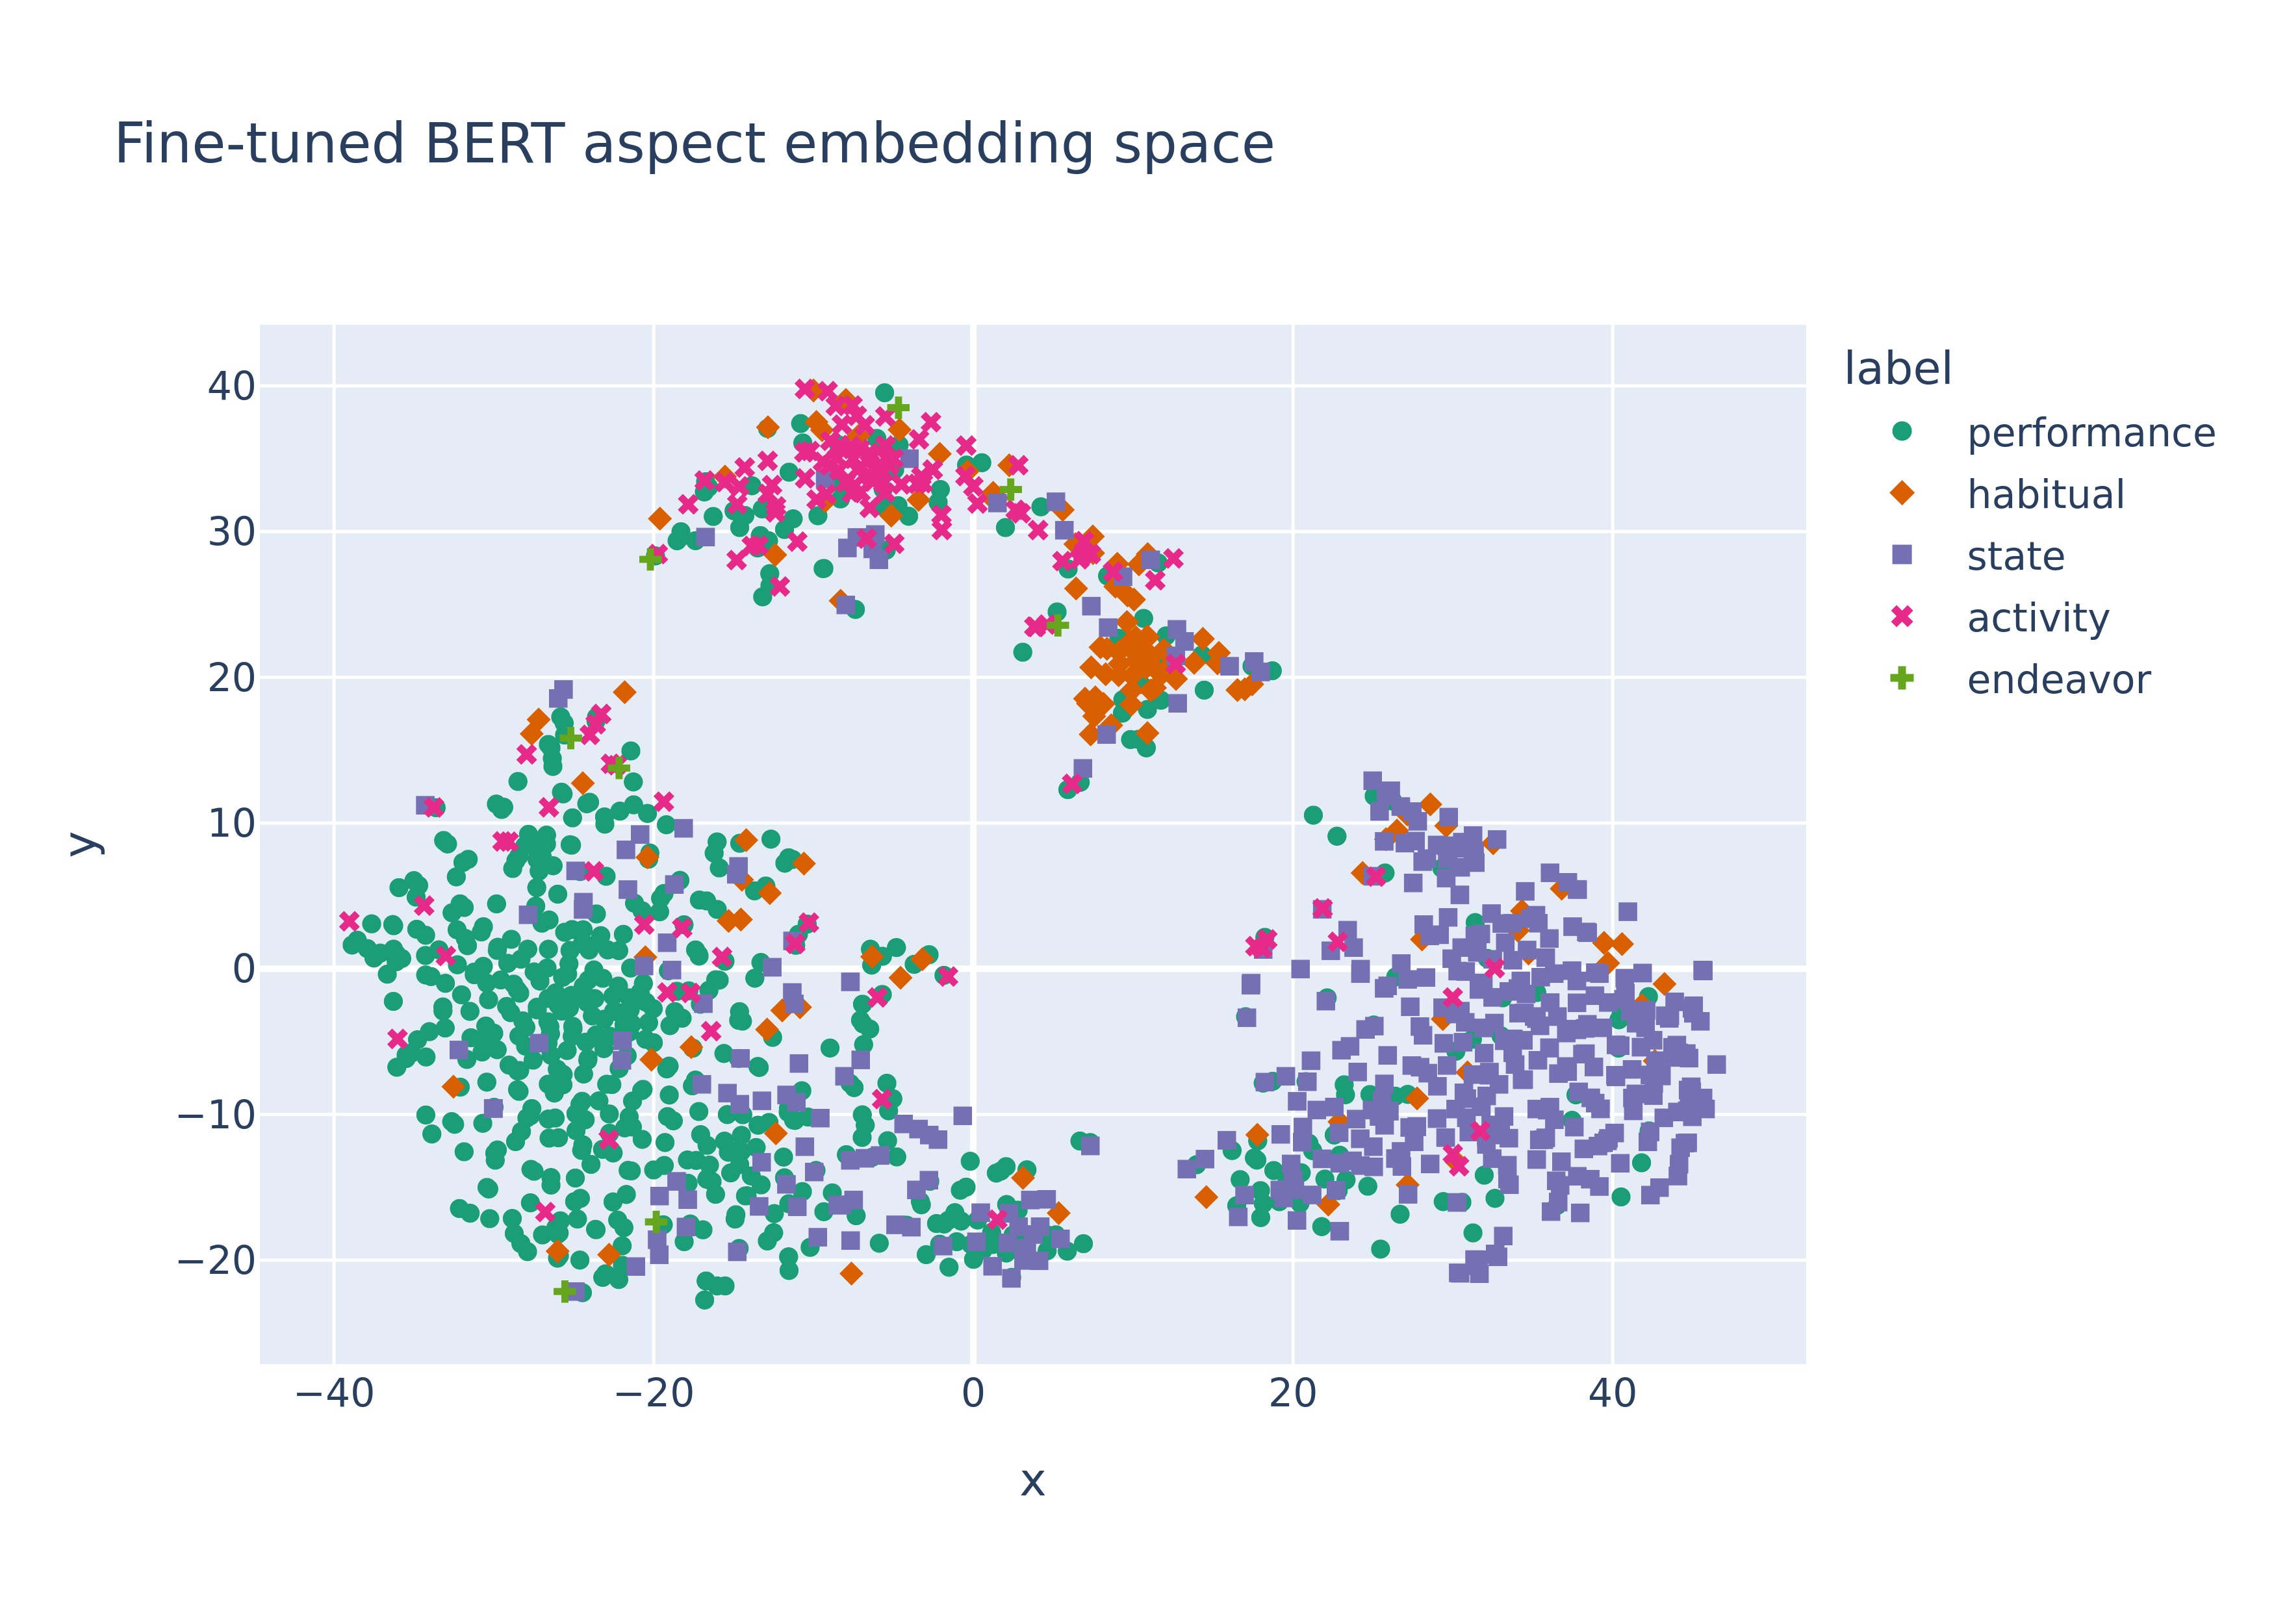
\includegraphics[width=\textwidth]{img/aspect_latent_space.jpeg}
    \caption{\texttt{[CLS]} embedding space of a BERT model fine-tuned on English verbs annotated for aspect in context, reduced to 2 dimensions by t-SNE.}
    \label{fig:fine-tuned_aspect_latent_space}
\end{figure}


\subsection{Multilingual BERT fine-tuning}
Since the LLM annotator Llama 3 can only be used in English, it is only possible to make training data in English. Luckily, however, there are multilingual models which can be trained with data using one language and then be used with languages other than that of the training data. I wanted to verify the performance of different models transferred to other languages and therefore needed a way of obtaining target labels for languages other than English.

I therefore trained a WHICH MODEL using WHICH DATASET annotated by the fine-tuned Llama 3 model and applied. The choice for this particular dataset was the availability of word-level alignments, a rarity in parallel corpora (IS THIS TRUE), meaning once a verb has been identified in the English sentence and given a particular aspect class, it is easy to find the corresponding verb in the other language. I only included sentences where the corresponding word in the other language is also a verb, since I wish to focus on verb phrases rather than general event classification.

In order to check the performance of this 

Get results in English and results in French

\begin{table}[h!]
    \centering
    \begin{tabular}{lcccc}
    \toprule
    \textbf{Model} & \multicolumn{2}{c}{\textbf{English}} & \multicolumn{2}{c}{\textbf{French}} \\
    \cmidrule(r){2-3} \cmidrule(r){4-5}
     & \textbf{F1 (best)} & \textbf{Acc} & \textbf{F1} & \textbf{Acc} \\
    \midrule
    \texttt{bert-base-multilingual-uncased} & 0.640 & 0.791 & 0.452 & 0.587 \\
    \texttt{bert-base-multilingual-cased}   & 0.647 & 0.790 & 0.450 & 0.572 \\
    \texttt{xlm-roberta-base}               & \textbf{0.665} & \textbf{0.813} & \textbf{0.522} & \textbf{0.651} \\
    \texttt{xlm-roberta-large}              & 0.647 & 0.797 & 0.447 & 0.629 \\
    \bottomrule
    \end{tabular}
    \caption{Model performance on English and French test sets after training on English training set.}
    \label{tab:performance}
    \end{table}

Hence, it is clear that the result is worse than in English, as is to be expected, however still significantly higher than chance.

\subsubsection{Russian aspect system}
As explained in \ref{sec:asp_in_slav_lang}


\subsubsection{Verb of motion clustering}
Unlike in English, almost all Russian imperfective verbs of motion have both a telic and an atelic counterpart. The former is used to describe a motion with a destination \ref{sent:telic_mv}, the latter for one without \ref{sent:atelic_mv}.

\begin{exe}
    \ex Ja \emph{šel} v školu. (I was walking to school.)
    \label{sent:telic_mv}
    \ex Ja \emph{chodil} po parku. (I was walking around the park.)
    \label{sent:atelic_mv}
\end{exe}

\begin{table}[h!]
    \centering
    \begin{tabular}{lllll}
    \textbf{Telic imperfective:} & Ja \emph{šel} v školu. &$\rightarrow $& \textsc{endeavour} & \checkmark\\
    \textbf{Telic perfective:} & Ja \emph{pošel} v školu. & $\rightarrow$ & \textsc{performance}  & \checkmark\\
    \textbf{Atelic imperfective:} & Ja \emph{guljal} po parku. & $\rightarrow$& \textsc{activity} & \checkmark\\
    \textbf{Atelic perfective:} & Ja \emph{poguljal} po parku. & $\rightarrow$& \textsc{activity} & ?\\
    \end{tabular}
    \caption{Model output of 3 example Russian sentences with motion verbs.}
    \label{tab:russian_mot_verb_outputs}
\end{table}

In UMR, events with no end goal are PROTOTYPISED? by activity, whereas telic events reaching completion are annotated with \texttt{performance}. We can verify that the model also makes this distinction HOW.

this empirically using the 

Using this we can 

\begin{table}[h!]
    \centering
    \begin{tabular}[t]{|l|c|c|r|l|}
        \hline
        \textbf{Verb} & & & \textbf{Entropy} & \textbf{PC} \\
        \hline
        schlappte &  &  & 0.00473 & performance\\
        schwebte &  &  & 0.00712 & activity\\
        trippelte &  &  & 0.00784 & activity\\
        schwankte &  &  & 0.00836 & activity\\
        schwamm &  &  & 0.00837 & activity\\
        pilgerte &  &  & 0.00856 & activity\\
        trabte &  &  & 0.00867 & activity\\
        strömten &  &  & 0.00877 & activity\\
        joggte &  &  & 0.00924 & activity\\
        flanierte &  &  & 0.00935 & activity\\
        tapste &  &  & 0.00943 & activity\\
        krabbelte &  &  & 0.00964 & activity\\
        watschelte &  &  & 0.0097 & performance\\
        latschte &  &  & 0.00996 & activity\\
        rutschte &  &  & 0.01028 & activity\\
        bummelte &  &  & 0.01128 & activity\\
        stromerten &  &  & 0.01148 & activity\\
        hüpfte &  &  & 0.01304 & activity\\
        purzelte &  &  & 0.01418 & activity\\
        schlurfte &  &  & 0.01443 & activity\\
        wanderte &  &  & 0.01623 & activity\\
        kullerte &  &  & 0.01686 & activity\\
        kroch &  &  & 0.01697 & activity\\
        hinkte &  &  & 0.01769 & activity\\
        schlich &  &  & 0.01799 & activity\\
        schweiften &  &  & 0.018 & activity\\
        streunten &  &  & 0.01959 & activity\\
        robbte &  &  & 0.01969 & activity\\
        wieselte &  &  & 0.0199 & activity\\
        glitt &  &  & 0.02027 & activity\\
        flatterte &  &  & 0.02123 & activity\\
        trampelte &  &  & 0.02399 & activity\\
        trieb &  &  & 0.0262 & activity\\
        hoppelte &  &  & 0.02664 & performance\\
        galoppierte &  &  & 0.02702 & activity\\
        wankte &  &  & 0.02801 & activity\\
        spazierte &  &  & 0.03137 & activity\\
        marschierte &  &  & 0.03802 & activity\\
        lief &  &  & 0.03966 & state\\
        reiste &  &  & 0.04599 & activity\\
        sprintete &  &  & 0.05367 & activity\\
    \end{tabular}
    \begin{tabular}[t]{|l|c|c|r|l|}
        \hline
        \textbf{Verb} & & & \textbf{Entropy} & \textbf{PC} \\
        \hline
        schlenderte &  &  & 0.05586 & activity\\
        tauchte &  &  & 0.05852 & activity\\
        hetzte &  &  & 0.06586 & activity\\
        ritt &  &  & 0.06784 & habitual\\
        taumelte &  &  & 0.07257 & activity\\
        trottete &  &  & 0.08606 & activity\\
        wandelte &  &  & 0.10565 & activity\\
        stolperte &  &  & 0.11249 & performance\\
        ruderte &  &  & 0.12711 & activity\\
        rannte &  &  & 0.13438 & activity\\
        tippelte &  &  & 0.1351 & performance\\
        torkelte &  &  & 0.13657 & activity\\
        tigerte &  &  & 0.16338 & activity\\
        skatete &  &  & 0.17054 & activity\\
        stieg &  &  & 0.17735 & endeavor\\
        humpelte &  &  & 0.18405 & activity\\
        radelte &  &  & 0.2051 & activity\\
        ging &  &  & 0.20655 & activity\\
        stapfte &  &  & 0.20949 & endeavor\\
        stapfte &  &  & 0.20949 & endeavor\\
        floh &  &  & 0.26129 & activity\\
        stolzierte &  &  & 0.33834 & activity\\
        huschte &  &  & 0.38448 & habitual\\
        fuhr &  &  & 0.39979 & performance\\
        raste &  &  & 0.40537 & activity\\
        kletterte &  &  & 0.44416 & habitual\\
        streifte &  &  & 0.49204 & activity\\
        hastete &  &  & 0.54362 & activity\\
        stürmte &  &  & 0.55842 & activity\\
        schritt &  &  & 0.5728 & performance\\
        eierte &  &  & 0.65506 & activity\\
        segelte &  &  & 0.67731 & activity\\
        sank &  &  & 0.74246 & performance\\
        sauste &  &  & 0.78209 & activity\\
        hopste &  &  & 0.78673 & endeavor\\
        flog &  &  & 0.84478 & activity\\
        flitzte &  &  & 0.85863 & activity\\
        rollte &  &  & 0.97166 & endeavor\\
        floss &  &  & 0.99165 & habitual\\
        sprang &  &  & 1.03842 & endeavor\\
        eilte &  &  & 1.27521 & activity\\
        \hline
    \end{tabular}
    \caption{CHANGE THIS}
\end{table}


\subsubsection{Prefix clustering}
An interesting application of this fine-tuned model is the 

ADD T-TEST FORMULA HERE

The probability of verbs with a prefix ($n=3489; \sigma = 0.3298; \mu = 0.1425$) being classified as the \textsc{state} class was lower than verbs without a prefix ($n=2473; \sigma = 0.4570; \mu = 0.3987$) by a statistically significant amount ($t = -25.1392; p < 1.3e-132$). This was also the case for the \textsc{activity} class, albeit by a much lesser degree ($t=-0.2841; p < 7.5e-2$). As can be seen in \ref{fig:fine-tuned_aspect_latent_space}, the opposite is also true for the \textsc{performance} class ($t=19.4150$), also with very high significance ($p<1.9e-081$). The differences between the \textsc{habitual} and \textsc{endeavour} classes was not significant.

This corroborates WHAT

\begin{figure}
    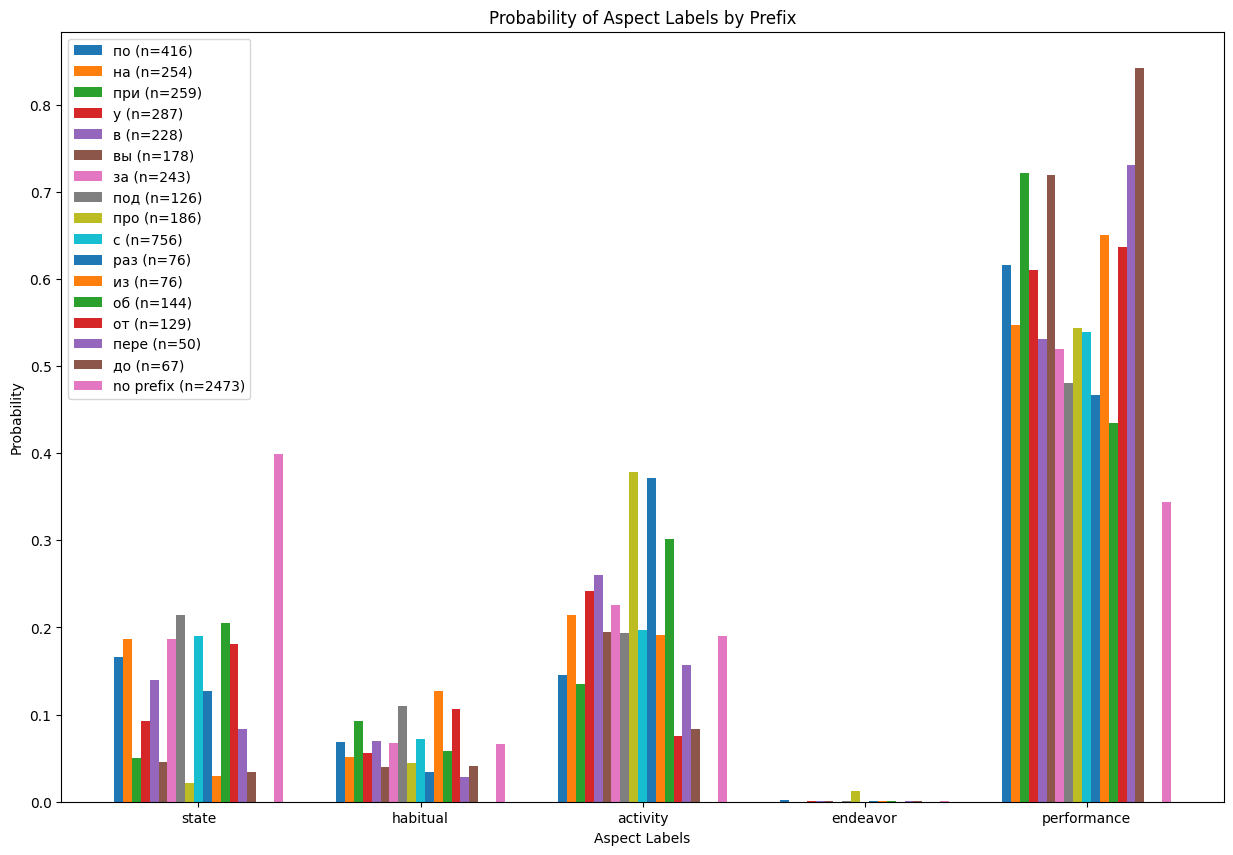
\includegraphics[width=\textwidth]{img/aspect_prediction_by_prefix.png}
    \caption{Look at this graph}
    \label{fig:fine-tuned_aspect_latent_space}
\end{figure}

Let's take the example of the prefixes \emph{pro-} (FIND OUT HOW TO ADD RUSSIAN HERE) and \emph{pere-}. While both meaning "through", they both emphasise different parts of the action. While \emph{pere-} simply implies that the "inceptive" and "terminal" limits of the domain being crossed have been traversed, \emph{pro-} puts emphasis on the action inside the domain and on the duration of this traversal \citep{0a0c5a60-a736-3226-b927-03ba8af4fd75}. This theoretical hypothesis is validated by the results here, with verbs beginning with \emph{pro-} exhibiting being classed significantly more often as \textsc{activity} ($t=3.2400; p<0.0014$).

both prefixes showing a significant difference in the 

\section{Aspectual ambiguity}
\subsection{Sentence-level ambiguity}
DOES ENTROPY CORRELATE WITH AMBIGUITY PREDICTION??
It is well known that LMs are often too confident of their predictions, even when wrong INSERT CITATION HERE

The first question that is interesting to ask (CHANGE DIESE FORMULIERUNG) is whether there is a correlation between the uncertainty of the aspect classification model and the output of the aspect ambiguity model, i.e. does a (supposed) ambiguous aspect reading of a sentence-verb pair correlate with uncertainty in the former's output. In order to quantify I take the concept of entropy and apply it to this case with the following formula:

$$H_{aspect} = - \sum_{i=1}^{\#AspClass}p(x_i)log(p(x_i))$$

In this way, higher uncertainty (i.e. a more balanced probability across all classes) leads to a higher $H_{aspect}$ value. It must be noted that this value is not comparable with models outputting a different number of classes (such as the traditional Vendlerian classification with 4), or indeed with different aspect classification systems (IS THIS TRUE??), however it serves the purpose for use to compare between languages (REWORD).

Using this value it is possible to calculate a correlation coefficient. The measure used was the point-biserial correlation coefficient, a metric mathematically equivalent to Pearson's correlation coefficient, however specialised for the case of one binary and one continuous variable. It is calculated thus:

$$r_{pb} = \frac{\overline{X}_1 - \overline{X}_0}{s} \sqrt{\frac{n_1 n_0}{n^2}}$$
where:
\begin{itemize}
    \item $\overline{X}_1$ is the mean of the continuous variable for the group where the binary variable is 1
    \item $\overline{X}_1$ is the mean of the continuous variable for the group where the binary variable is 0
    \item $s$ is the standard deviation of the continuous variable
    \item $n_1$ is the number of observations in the group where the binary variable is 1
    \item $n_0$ is the number of observations in the group where the binary variable is 0
    \item $n$ is the total number of observations
\end{itemize}

I found that the model entropy value had a \emph{medium}\footnote{According to Cohen's interpretation of Pearson's correlation \citep{cohen1988spa}} correlation of $\rho = 0.3465$ ($p < 0.0006$) with the upsampled ambiguity data derived from the human annotations. This is an encouraging result, especially the significance, however the correlation is not particularly high, and we should expect this value to be even lower for languages other than English, which sadly decreases the reliability of any conclusions taken from using the entropy value of this model. Furthermore, there was no correlation with the annotations of the fine-tuned LLM ($\rho = 0.0028; p < 0.85$), which is a disappointing result. 

Nevertheless, while this correlation with human is too small to lead to meaningful results on the level of individual datapoints, with a large enough sample size we can still use this to find general tendencies on the macro level, such as at language level.

\subsection{Verb-level ambiguity (TAKE OUT?)}

\subsection{Language-level ambiguity: Cross-linguistic comparison}

In order to compare between languages, it is first necessary to find a corpus available in the all the languages I wish to compare, if not parallel then with at least similar texts. To this end I decided to use TED2013 IS THIS TRUE???? corpus

Since I am comparing verbal ambiguity, I wished to 
